\documentclass[psamsfonts,onesided,10pt,letterpaper]{amsart}%

%\usepackage{hyperref}

\input{commands.tex}%

%\usepackage{fullpage}



\usepackage{showkeys}%
\usepackage{todonotes}

\author{Peter Bonventre, Lu\'is Alexandre Pereira}%
\title{Coloured Model Structure Using Interval Objects}%
\date{\today}



%-------- TIKZ -----------------------------------------
\usepackage{tikz}%
\usetikzlibrary{matrix,arrows,decorations.pathmorphing,
cd,patterns,calc}
\tikzset{%
  treenode/.style = {shape=rectangle, rounded corners,%
                     draw, align=center,%
                     top color=white, bottom color=blue!20},%
  root/.style     = {treenode, font=\Large, bottom color=red!30},%
  env/.style      = {treenode, font=\ttfamily\normalsize},%
  dummy/.style    = {circle,draw,inner sep=0pt,minimum size=2mm}%
}%

\usetikzlibrary[decorations.pathreplacing]

% -------------------- new commands --------------------


\renewcommand{\C}{\ensuremath{\mathfrak{C}}}
\renewcommand{\fc}{\ensuremath{\mathfrak{c}}}
\newcommand{\FF}{\ensuremath{\mathbb{F}}}
\renewcommand{\H}{\ensuremath{\mathbb{H}}}
\newcommand{\I}{\ensuremath{\mathbb{I}}}
\newcommand{\J}{\ensuremath{\mathbb{J}}}
%\newcommand{\1}{\ensuremath{\mathbf{1}}}
\renewcommand{\P}{\ensuremath{\mathcal{P}}}
\newcommand{\Q}{\ensuremath{\mathcal{Q}}}
% \newcommand{\V}{\mathcal V}
\newcommand{\Vsigma}{\ensuremath{\V^{\Stab(\sigma)}_{\F_\sigma}}}
\newcommand{\N}{\mathbb N}


\newcommand{\floor}[1]{\left \lfloor #1 \right \rfloor}
%\newcommand{\dasharrowdbl}{\dashrightarrow\mathrel{\mkern-14mu}\dashrightarrow}
%\newcommand{\xdasharrowdbl}[2][]{%
%  \xdashrightarrow[#1]{#2}\m}
%\newcommand{\tall}[2]{\ensuremath{\begin{tikzcd} #1 \arrow[r,dashed,twoheadrightarrow] & #2 \end{tikzcd}}}
\newcommand{\tall}{\ensuremath{\Rightarrow}}%\rightsquigarrow
\newcommand{\Tall}{\ensuremath{\Downarrow}}%\rightsquigarrow

\newcommand{\T}{\ensuremath{\mathbb{T}}}

\newcommand{\iso}{\ensuremath{\mathsf{Iso}}}
\newcommand{\alt}{\ensuremath{\mathsf{alt}}}


% \newcommand{\Cat}{\mathsf{Cat}}
% \newcommand{\Op}{\mathsf{Op}}
%\renewcommand{\Sym}{\mathsf{Sym}}
% \newcommand{\Stab}{\mathrm{Stab}}

\newcommand{\Omeganc}{\ensuremath{\Omega_{(n-1,1)-\mathfrak c}}}
\newcommand{\Omeganbin}{\ensuremath{\Omega_{(n-1,1)-bin}}}
\newcommand{\Omeganalt}{\ensuremath{\Omega_{(n-1,1)-alt}}}

\setenumerate[0]{label=(\arabic*)}
\newcommand{\primed}[1]{$#1 '$}

\begin{document}		\maketitle%

%\tableofcontents

\section{Introduction}%
%$\dashrightarrow$
%$\dasharrowdbl$
%$\twoheadrightarrow$
%$\tall{A,B}$
%\begin{tikzcd} A \arrow[r,dashed,twoheadrightarrow] & B \end{tikzcd}

\[
	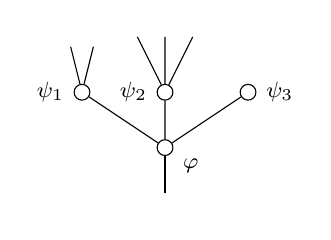
\begin{tikzpicture}[grow=up, every node/.style = {font=\footnotesize},level distance = 2em]%
	\tikzstyle{level 2}=[sibling distance=3em]%
	\tikzstyle{level 3}=[sibling distance=1em]%
		\node {}%
			child{node [dummy,label=-10:$\varphi$] {}%
				child{node [dummy,label=right:$\psi_3$] {}}%
				child{node [dummy,label=left:$\psi_2$] {}%
					child{}%
					child{}%
					child{}%
				}%
				child{node [dummy,label=left:$\psi_1$] {}%
					child{node {} }%
					child{node {} }%
				}%
			};%
	\end{tikzpicture}%
\]%


We recall a particular description of operads and their equivariant generalizations, and define a new category of ``genuine equivariant operads'' which forget to highly structured coefficient systems of (non-equivariant) operads. We define model structures on both of these categories, and show that there are natural functors realizing a Quillen equivalence.


\begin{definition}
      For a category $\V$, a {\em Hopf interval object} in is a cofibrant Hopf object $\H\in\V$ for which there exists a factorization
      $\begin{tikzcd} 
            I\coprod I \arrow[r,rightarrowtail] & \H \arrow[r, twoheadrightarrow, "\simeq"] & I
      \end{tikzcd}$ 
      of the fold map $I$, the unit in $\V$. We can $\H$ {\em cocommutative} if its Hopf structure is. 
\end{definition}

\begin{definition}
      Similarly but different: let $\I$ be the $\V$-category with objects $\set{0,1}$ with $\I(0,0) = \I(0,1) = \I(1,0) = \I(1,1) = 1_V$. A {\em $\V$-interval} is a cofibrant object in $\V\Cat_{\set{0,1}}$ (with the transfered model structure) weakly equivalent to $\I$. A set $\mathcal{G}$ of $\V$-intervals is {\em generating} if all $\V$-intervals $\J$ can be obtained as a retract of a trivial extension of an element in $\mathcal{G}$ in $\V\Cat_{\set{0,1}}$:
\[
\begin{tikzcd}
  \mathbb{G} \arrow[r,rightarrowtail, "\simeq"] & \mathbb{K} \arrow[r,yshift=-.3em, "r"'] & \mathbb{J} \arrow[l,yshift=.3em, "i"']
\end{tikzcd}
\]
\end{definition}

\subsection{Assumptions}

We assume the following conditions on the enriching category $\V$:

\begin{enumerate}
\item $\V$ strongly cofibrantly generated monoidal model category;
\item $G\V$ and $G\V Cat$ have cellular fixed point functors for all finite groups $G$;
\item $\V$ satisfies transfer for symmetric operads (in particular if $\V$ has a cofibrant unit, has a cocommutative Hopf interval object (in particular, cartesian closed \cite{BM03}), and admits a monoidal fibrant replacement functor \cite{BM07});
\item $\V$ admits a symmetric monoidal fibrant replacement functor which commutes with $H$-fixed points: $R(X)^H = R(X^H)$. 
\end{enumerate}

Additionally, we may assume
\begin{enumerate}
%\item $\V^G_\F$ has a symmetric monoidal fibrant replacement functor for any finite group $G$ and family of subgroups $\F$;
\item $\V Cat$ has a generating set of intervals;
\item $\V$ is right proper
\item $W$ (to be defined later) is closed under transfinite compositions.
\end{enumerate}

Most of the results will not need all of these assumptions, but this is the most we could possibly require (I think). I will label each result by what is needed (if possible).

Let $I$ and $J$ be the sets of generating cofibrations and generating trivial cofibrations of $\V$.

 \todo[inline]{STUFF}

\newpage
\section{Equivariant operads}

STuff

\subsection{Operads of equivariant operads}

Given a $G$-set $\C$, we define a colored operad $\Op_\C$ whose algebras are $G$-operads with colors $\C$.

The colors of $\Op_\C$ are pairs $(C,\fc)$ with $C$ a corolla, and $\fc: E(T) \to \C$ a set map.

Morphisms are generated by two types of maps:
\begin{enumerate}
\item $(T,\fc,\sigma,\set{\phi_i},\tau)\in \Op_\C((C_1,\fc_1), \ldots, (C_n,\fc_n); (C_0,\fc_0))$, where
  \begin{itemize}
  \item $T$ is a tree with $n$ vertices;
  \item $\fc: E(T)\to \C$ is a set math with $\fc(L(T)) = \fc_0(L(C_0))$ and $\fc(r) = \fc_0(r)$;
  \item $\sigma: \set{1,\ldots, n}\to V(T)$ a bijection such that, if $C[\sigma(i)]$ is the corolla in $T$ connectd to the vertex $\sigma(i)$, we have isomorphisms of colored corollas $\phi_ii: (C[\sigma(i)], \fc|_{C[\sigma(i)]})\xrightarrow{\cong} (C_i, \fc_i)$ for all $i\in \set{1,\ldots, n}$;
  \item $\tau: L(C_0)\to L(T)$ a bijection such that $\fc\tau = \fc_0$;
  \end{itemize}
\item $g\in \Op_\C((C,\fc); (C,g\fc))$
\end{enumerate}
modulo the relation $(T,\fc,\sigma,\set{\phi_i},\tau) = (T,\fc\pi^{-1},\pi\sigma,\set{\pi\phi_i},\pi\tau)$ for all $\pi\in \mathrm{Aut}(T)$.

Composition is defined as follows:
\begin{enumerate}
\item $[T,\fc,\sigma,\set{\phi_i},\tau] \circ_j [S,\mathfrak{d}, s, \set{\psi}, t] = [T\circ_{\sigma(j)}S, \fc', \sigma', \set{\phi_i}\amalg\set{\psi_{\sigma' i}}, \tau']$ where, if $T$ has $n$ vertices and $S$ and $m$ vertices, we have defined
\[
\fc'(e) = \begin{cases}\fc(e) & e\in T\\ \mathfrak{d}(e) & e\in S\end{cases} \qquad \mbox{and} \qquad 
\sigma'(i) =
\begin{cases}
  \sigma(i) & i< j\\
  s(i-j)+j & j\leq i < j+m\\
  \sigma(i-m)+m & i\geq j+m
\end{cases}
\]
and $\tau'$ synthesizes $\tau$ and $t$ (if neceesary) to retain the identification information on the leaves;
\item $g\circ h = gh$;
\item composition between $g$ and $[T]$ is free modulo
\[
[T,\fc,\sigma,\set{\phi_i},\tau] \circ (g,\ldots,g) = g\circ [T,g\fc,\sigma,\set{\phi_i}, \tau].
\]
\end{enumerate}

\newpage
\section{Model stucture on the category of equivariant operads}

\begin{proposition}[\cite{Stephan16}, 2.6]
  Assume $\V$ is cofibrantly generated model category such that $G\V$ has cellular fixed points for all finite groups $G$, and let $\F$ be any family of subgroups of $G$. Then $\V^G$ has the $\F$-model structure; that is, $\V^G$ has a cofibrantly generated model structure where weak equivalences and fibrations are defined by $(-)^H$ for all $H\in \F$. In particular, the generating cofibrations $I_\F = \sets{G/H\otimes i}{i\in I,\ H\in \F}$ and the generating trivial cofibrations $J_\F = \sets{G/H\otimes j}{j\in J,\ H\in \F}$. 
\end{proposition}

Now, let $G$ be a finite group, and suppose we have an {\em indexing family} $\F = \set{\F_n}$ of families of subgroups of $\set{G\times \Sigma_n}$ (c.f. \cite{BH15}). 

Let $\C$ be a $G$-set, of {\em colors}, and $Seq(\C)$ be the set of {\em signatures} in $\C$, defined by
$\sets{
  (a_1,\ldots, a_n; a)\in \C^n\times\C
}
{n\in\mathbb{N}}$.
For each $n$, the set of signatures of length $n+1$ have an action by $G\times \Sigma_n$, where $G$ acts on all components, and $\Sigma_n$ acts on all but the last one. 


\begin{definition}
  Let $\V Op^G_\C$ be the category of $\C$-colored $\V$-operads.
\end{definition}

\begin{lemma}
  For each $G$-set $\C$, we have a monoidal free-forgetful adjunction as below;
\[
\begin{tikzcd}
      fgt: \V Op^G_\C \arrow[r,yshift=-.3em, "\perp"]
      &
      \displaystyle\prod_{n\in\N}\displaystyle\prod_{[\sigma]\in\Sym_n(\C)/G\times\Sigma_n}\V^{\Stab(\sigma)}
      \arrow[l, yshift=.3em]
      : \FF_\C
\end{tikzcd}
\]
\end{lemma}

Given a signature $\sigma$ of length $n+1$, define $\F_\sigma$ to be the family of subgroups $\Lambda\in \F_n$ such that $\Lambda\leq \Stab(\sigma)$.
\begin{corollary}
  For any such $\sigma\in Seq(\C)$ and family $F_n$, $\V^{\Stab(\sigma)}$ has the $\F_\sigma$-model structure.
\end{corollary}

\begin{proposition}
  Suppose $\V$ cartesian closed monoidal model category with cartesian unit and cocommutative Hopf interval object, such that $\V^{\Stab(\sigma)}_{\F_\sigma}$ has a symmetric monoidal fibrant replacement functor which commutes with fixed points. Then the free-forgetful adjunction $(fgt, \FF)$ above 
% \[ 
% \begin{tikzcd}
%   fgt: \V Op^G_\C \arrow[r,yshift=-.3em, "\perp"] & \displaystyle\prod_{n\in\N}\displaystyle\prod_{[\sigma]\in\Sym_n(\C)/G\times\Sigma_n}\V^{\Stab(\sigma)} \arrow[l, yshift=.3em] : \FF_\C
% \end{tikzcd}
% \]
induces a transfered model structure on $\V Op^G_\C$.
\end{proposition}
\begin{proof}
      We use the same arguments as in \cite{BM03}, Theorem 3.2. In particular, we know that $fgt$ preserves filtered colimits. Moreover, given $\O\in \V Op^G_\C$, define $\tilde \O$ by $\tilde \O(\sigma) = R\O(\sigma)$, where $R$ is the fibrant replacement functor in $\V$; since $R$ commutes with fixed points, this is in fact a levelwise fibrant replacement ($(\O_f)^H = (\O^H)_f$). Further, since $R$ is symmetric monoidal, the operad structure on $\O$ induces one of $\tilde \O$.
      {\color{red}
        Lastly, we need a functorical path object in $\V Op^G_\C$. Since $\V$ cartesian monoidal, given any cocommutative Hopf interval object $\H$ , and fibrant $\O$, we have 
        \[
              \begin{tikzcd}
                    \O \cong \O^I \arrow[r,"\simeq"] & \O^\H \arrow[r,twoheadrightarrow] & \O^{I\coprod I} \cong \O\times \O
              \end{tikzcd}
        \]
        for which the first arrow (resp. second arrow) is a cofibration (resp. fibration) by the pushout-product axiom of monoidal model categories, since $I$ is cofibrant. Lastly, these are (maps of) operads since $\V$ cartesian closed.
      } % color red
      \todo[inline]{the red above is quite wrong.}
\end{proof}

\begin{definition}
  Let $G\V Op$ be the category of $\V$-operads with any coloring $G$-set, where a map $F: \O\to \P$ is defined by a map of colors $f: \C(\O)\to \C(\P)$, and then a map $F: \O\to f^*\P$, where $f^*P(\sigma) = P(f(\sigma))$. Equivalently, $G\V Op$ is the category of $G$-objects in $\V Op$. 
\end{definition}

We have another free-forgetful adjunction $j^*: G\V Op \leftrightarrow G\V Cat: j_!$, and note that $j^*$ commutes with taking $H$-fixed points for all $H\leq G$;
\[
\begin{tikzcd}
  G\V Op \arrow[d, "(-)^H"] \arrow[r, yshift=-.3em, "j^*"', "\perp"] & G\V Cat \arrow[l, yshift=.3em, swap, "j_!"] \arrow[d, "(-)^H"] \\
  \V Op \arrow[r, yshift=-.3em, "j^*"', "\perp"] & \V Cat \arrow[l, yshift=.3em, swap, "j_!"]
\end{tikzcd}
\]

\begin{definition}
  We call a map $F: \O \to \P$ in $G\V Op$
  \begin{itemize}
  \item a {\em local fibration} (resp. {\em local weak equivalence}) if $F(\sigma): \O(\sigma)\to F^*\P(\sigma)$ is a fibration (resp. weak equivalence) in $\V^{\Stab(\sigma)_{\F_\sigma}}$ for all $\sigma\in Sig(\C(\O))$;
  \item a {\em local trivial fibration} if both a local fibration and a local weak equivalence;
  \item {\em essentially surjective} (resp. {\em path lifting}) if $j^*F^H$ is essentially surjective (resp. path lifting) in $\V Cat$ for all $H\leq G$;
  \item a {\em fibration} if both path-lifting and a local fibration
  \item a {\em weak equivalence} if both essentially surjective and a local weak equivalence.
  \end{itemize}
\end{definition}

\subsection{Generating (Trivial) Cofibrations and Local Fibrations}

We generalize and combine efforts from \cite{CM1, BM13, Cav14}.

Given $X\in \V^{\Stab(\sigma)}$, define $\iota_\sigma X\in \prod_n\prod_{[\sigma]}\Vsigma$ to be the collection defined by
\[
\iota_\sigma X(\tau) =
  \begin{cases}
    g*\tau & \tau = g.\sigma\\
    \varnothing & \mbox{else}
  \end{cases}
\]
where we have chosen a bijection $G\sigma \to G/\Stab(\sigma)$, and $\varnothing$ is the initial object in $\V$. This is natural in $X$, and in fact is the left adjoint to $p_\sigma$, the functorial projection onto the $\sigma$-th component. 

Let $\C_\sigma$ be the subset of $\C$ given by the the $G$-closure of the component elements in $\sigma$, and define $\FF_\sigma[X]\in G\V Op$ to be the composite $\FF_{\C_\sigma}\iota_\sigma X$.

\begin{lemma}[c.f. \cite{CM1} 1.16]
  $F: \O \to \P$ in $G\V Op$ has the right lifting property against $\FF_\sigma[X]\to \FF_\sigma[Y]$, $X,Y\in\Vsigma$, {\sc iff} $\O(\tau)\to\P(\tau)$ have the right lifting proeprty against $X\to Y$ for all $\tau\in Seq(\C)$ such that $\Stab(\tau)\geq \Stab(\sigma)$.  
\end{lemma}
\begin{proof}
  This follows from a string of equivalences of lifting diagrams. Since $\C(\FF_\sigma[X]) = \C(\FF_\sigma[Y])= \C_\sigma$, a lift of $F:\O\to \P$ against $\FF_\sigma[a]: \FF_\sigma[X]\to\FF_\sigma[Y]$ is equivalent to a lifting diagram of $a^*F: a^*\O \to a^*F^*\P$ against $\FF_\sigma[a]$, which is itself equivalent to a lift of $fgt(a^*F)$ against $\iota_\sigma a$. Lastly, this is equivalent to a lift of form
\[
\begin{tikzcd}
  X \arrow[r] \arrow[d,"a"] & \O(a(\sigma)) \arrow[d, "F(a(\sigma))"] \\
  Y \arrow[r] \arrow[ur, dotted] & \P(aF(\sigma))
\end{tikzcd}
\]
in $\V^{\Stab(\sigma)}$. Thus $F$ having right lifts against $\FF_\sigma[a]$ is precisely the same as $F(\tau)$ having lifts in $\V^{\Stab(\sigma)}$ against $a$ for all possible images $\tau = a(\sigma)\in Seq(\C(\O))$ of $\sigma\in Seq(\C_\sigma)$; these are precisely those signatures such that $\Stab(\tau)\geq \Stab(\sigma)$. 
\end{proof}

Given subgroups $H\leq K \leq G$ and a homomorphism $\rho: H\to \Sigma_n$ for $H\leq G$, let $\C_{n,\rho,K}$ be the $G$-set given by $C_{n,\rho,K} = G\times_H\set{1,2,\ldots, n} \coprod G/K\cdot \set{0}$ where $\rho$ determines the $H$-set structure on $\set{1,\ldots, n}$. Let the collection of all such $\C_{n,\rho,K}$ as $n$, $\rho$, and $K$ vary, modulo the natural $G\times \Sigma_n$-action, be denoted $\C_G$.

Define $I_{loc}$ to be the set $\sets{\FF_\sigma(i_\sigma)}{\mbox{$\sigma\in\C_{n,rho,K}$ for some $C_{n,\rho,K}\in \C_G$, $i_\sigma\in I_\sigma$}}$, where $I_\sigma$ is the collection of generating cofibrations of $\V^{\Stab(\sigma)}$.

Similarly, define $J_{loc}$ to be the set $\sets{\FF_\sigma(j_\sigma)}{\mbox{$\sigma\in\C_{n,rho,K}$ for some $C_{n,\rho,K}\in \C_G$, $j_\sigma\in J_\sigma$}}$, where $J_\sigma$ is the collection of generating trivial cofibrations of $\V^{\Stab(\sigma)}$. 

As a direct corollary of the above proposition, we have:
\begin{corollary}[c.f. \cite{Cav14} Section 4.2, \cite{CM1} 1.16]
  $\O\to \P$ is a local fibration {\sc iff} $\O\to \P$ has the right lifting property against $J_{loc}$.
  
  Similarly, $\O\to \P$ is a local trivial fibration {\sc iff} $\O\to \P$ has the right lifting property against $I_{loc}$.  \qed
\end{corollary}

Now, define $I_{GVOp}:= I_{loc} \cup \sets{\varnothing \to G/H\otimes \1}{H\leq G}$ and $J_{GVOp} := J_{loc} \cup \sets{G/H\otimes \1 \to G/H\otimes \J}{H\leq G,\ \J\in\mathbb{G}}$ where again $\1$ is the initial $\V$-category (thought as an operad), and $\mathbb{G}$ is a generating set of $\V$-intervals. 

We claim these are generating cofibrations and trivial cofibrations:
\begin{lemma}
  \label{CAV_4.8}
  [c.f. \cite{Cav14} 4.8, \cite{BM13} 2.3, \cite{CM1} 1.18]
  A map $F$ in $G\V Op$ is a trivial fibration {\sc iff} $F$ is a local trivial fibration such that $F^H$ is surjective on $H$-fixed colors for all $H\leq G$ {\sc iff} $F$ has the right lifting property against $I_{GVOp}$.. 
\end{lemma}
\begin{proof}
  By definition, $F$ is a trivial fibration {\sc iff} it is a local trivial fibration such that $j^*F^H$ is path-lifting and essentially surjective for all $H\leq G$. Thus, \cite{Cav14} 4.8 immediately implies the first step. Moreover, right lifting against $I_{loc}$ is identical to being a local trivial fibration, while lifting against $\varnothing \to G/H\otimes \1$ precisely say that $F^H$ is surjective on colors; combining these observations, we get our result.
\end{proof}

\begin{lemma}
  [c.f. \cite{CM1} 1.20, \cite{Cav14} Section 4.3]
  $F$ has right lifting against $J_{GVOp}$ {\sc iff} $F$ is a local fibration such that $F^H$ is path lifting for all $H\leq G$.
\end{lemma}
\begin{proof}
  Again, lifting against $J_{loc}$ is identical to being a local fibration, while lifting against $G/H\otimes \1 \to G/H\otimes \J$ (that is, $F^H$ has lifting against $\1\to \J$) implies that $F^H$ is path lifting by \cite{Cav14}. 
\end{proof}

Thus our definitions of ``fibration'' and ``trivial fibration'' match our generating sets of maps. Moreover
\begin{lemma}
  \label{POINT_4_LEMMA}
  [c.f. \cite{CM1} 1.19]
  $J_{GVOp}-cof \subseteq I_{GVOp}-cof$; that is, the set of trivial cofibrations sits inside the set of cofibrations.
\end{lemma}
\begin{proof}
  It suffices to show that if $F$ has right lifting against $I_{GVOp}$, it has right lifting aginst $J_{GVOp}$. Obviously, a local trivial fibration is a local fibration. On the other hand, by locality, any cofibration in $G\V Op_\C$ for any $\C$ includes to a cofibration in $G\V Op$. Hence, since $G/H\otimes \1 \to G/H\otimes \1 \coprod G/H\otimes \1$ is in $I_{GVOp}-cof$, the composition
$
\begin{tikzcd}
 G/H\otimes \1 \arrow[r, rightarrowtail] & G/H\otimes \1 \coprod G/H\otimes \1 \arrow[r, rightarrowtail, "\simeq"] & G/H\otimes \J 
\end{tikzcd}
$
is in $I_{GVOp}-cof$. Thus $J_{GVOp}-cof \subseteq I_{GVOp}-cof$, as desired.
\end{proof}

\subsection{Trivial cofibrations are weak equivalences}

\begin{lemma}
  The transfinite composition of essentially surjective maps is essentially surjective.
\end{lemma}
\begin{proof}
  Since taking fixed points commutes with filtered colimits, they commute with transfinite composition, and hence by \cite{Cav14} 4.17, we are done.
\end{proof}

\begin{lemma}
  \label{J-CELL_LEMMA}
  [c.f. \cite{Cav14} 4.20]
  If weak equivalences are closed under transfinite compositions, then relative $J_{GVOp}$-cells are weak equivalences. 
\end{lemma}
\begin{proof}
  Since local weak equivalences are closed under transfinite composition by assumption, and essentially surjective maps are closed under transfinite composition by the above lemma, it suffices to prove that the pushout of a map $j\in J_{GVOp}$ is weak equivalences. If $j\in J_{loc}$, then since colimits in $G\V Op$ are computed in $\V Op$, and since by \cite{Cav14} pushouts of this form can be computed fiberwise (that is, after shifting the operads into a single color), we are computing the pushout of a trivial cofibration in $G\V Op_{\C_{\sigma}}$, which by the existance of the tranfsered model structure there is again a trivial cofibration. Hence, the pushout is a local weak equivalence in $G\V Op$ which is the identity on colors, and hence a weak equivalence itself.

Now, supppose $j = G/H\otimes \1 \to G/H\otimes \J$ for $\J$ a $\V$-interval. As in \cite{Cav14}, we can split this pushout into a composition of two pushouts
\[
\begin{tikzcd}
  G/H\otimes \1 \arrow[r] \arrow[d, "G/H\otimes \phi"'] \arrow[dr,phantom, yshift=.1em, xshift=.5em, "\lrcorner" near end] & X \arrow[d,"\phi'"] \\
  G/H\otimes \J_{\set{0,0}} \arrow[r] \arrow[d, "G/H\otimes \psi"'] \arrow[dr,phantom, yshift=.1em, xshift=.5em, "\lrcorner" near end] & X' \arrow[d,"\psi'"]\\
  G/H\otimes \J \arrow[r] & Y
\end{tikzcd}
\]
where $\J_{\set{0,0}}$ is the full subcategory of $\J$ spanned by the object $O$. It suffices to show both $\psi'$ and $\phi'$ are local weak equivalences which are essentially surjective on fixed points. 

Now, we know \cite{Cav14} that $\psi$ is injective on colors and fully-faithful (that is, induces an isomorphism in $\V Op_{\set{0}}$) and hence $G/H\otimes\psi$ is also injective on colors and fully-faithful as a map in $\V Op$. Since colimits are created non-equivariantly, by \cite{Cav14} Proposition B.22 and the remark thereafter, we conclude that $\psi'$ is fully faithful in $\V Op$, and hence is an isomorphism in $\V Op_{\C(X')}$. But $\psi'$ is a $G$-map, and hence it is an isomorphism in $G\V Op_{\C(X')}$ as well, and hence is a local weak equivalence in $G\V Op$. 

Moreover, we observe that $\C(Y) = \C(X')\coprod G/H\times \set{1}$. Thus, if $x\in \C(Y)^K$ is in $\C(X')$, we have essential surjectivity trivially:
\[
\begin{tikzcd}
   \1 \arrow[rrr, "x"] \arrow[dr, " i_0"] &&& (X')^K \arrow[dd, "\psi'"] \\
  &  \J \arrow[r] &  \1 \arrow[dr, "x"] \\
   \1 \arrow[ur, " i_1"] \arrow[rrr,"x"] &&& (Y)^K
\end{tikzcd}
\]
Lastly, if we consider any orbit of the new object $1\in \C(Y)$, there is an associated object $0\in\C(X')$ such that the essentially surjectivity diagram is the same as the pushout diagram for $\psi$:
\[
\begin{tikzcd}
  G/H\otimes \1 \arrow[rr,"0"] \arrow[dr, "G/H\otimes i_0"] & & X' \arrow[dd, "\psi'"]\\
  & G/H\otimes \J \arrow[dr, "\mbox{\large $\lrcorner$}" near end] \\
  G/H\otimes \1 \arrow[ur, "G/H\otimes i_1"] \arrow[rr, "1"] && Y
\end{tikzcd}
\]
Hence $\psi'$ is essentially surjective and a local weak equivalence, hence a weak equivalence in $G\V Op$. 

Similarly, when considering $\phi'$, \cite{Cav14} 4.20 again says that pushouts of this form are created in $\V Op_{\C(X)}$ as the pushout
\[
\begin{tikzcd}
  p_! G/H\otimes \1 \arrow[r, "p"] \arrow[d, "p_!G/H\otimes \phi"] & X \arrow[d,"\phi'"] \\
  p_! G/H\otimes \J_{\set{0,0}} \arrow[r] & Y
\end{tikzcd}
\]
In particular, this implies $\phi'$ is bijective on objects, and hence essentially surjective. Moreover, as $\phi$ is a trivial cofibration in $\V Op$ \cite{Cav14}, $p_!G/H\otimes \phi$ is a trivial cofibration in $G \V Op_{\C(X)}$. Thus $\phi'$ is a trivial cofibration in $G\V Op_{\C(X)}$, and thus is a local weak equivalence in $G \V Op$.

Hence both $\phi'$ and $\psi'$ are weak equivalences in $G\V Op$, so the result is proved.
\end{proof}

\subsection{2-out-of-3}

We recall some equivalence relations on objects in a $\V$-category \cite{Cav14, BM13}:
\begin{definition}
  Given $\mathcal{C}$ in $\V\Cat$ and $a,b\in\mathrm{Ob}{\mathcal C}$, we say $a$ and $b$ are
  \begin{itemize}
  \item {\em equivalent} if there exists a map $\gamma: \J \to \mathcal C$ such that $\gamma i_0 = \set{a}$ and $\gamma i_1 = \set{b}$ for some $\V$-interval $\J$;
  \item {\em virtually equivalent} if $a$ and $b$ are equivalent in some fibrant replacement $\mathcal C_f$ of $\mathcal C$ in $\V\Cat_{\mathrm{Ob}(\mathcal C)}$;
  \item {\em homotopy equivalent} if there exist maps $\alpha: 1_\V \to \mathcal C_f(a,b)$ and $\beta: 1_\V\to \mathcal C_f(b,a)$ such that $\beta\alpha$ and $\alpha\beta$ and homotopic to the identity arrows $1_V\to \mathcal C_f(a,a)$ and $1_V\to\mathcal C_f(b,b)$, respectively. Equivalently, if $a$ and $b$ are isomorphic in the 1-category $\pi_0\C_f = \mathrm{Ho}\V(1_\V, \mathcal C_f)$.
  \end{itemize}
\end{definition}

We equivariantize these definitions to $G\V\Cat$ and $G\V Op$:
\begin{definition}
  Given $\mathcal{C}\in G\V\Cat$ and $a,b\in \mathrm{Ob}(\mathcal{C})$, we say $a$ and $b$ are
\begin{itemize}
\item {\em equivalent} if $\Stab_G(a) = \Stab_G(b) =: H$ and are equivalent in $\mathcal{C}^H$;
\item {\em virtually equivalent} if they are equivalent in some fibrant replacement $\mathcal{C}_f$ of $\mathcal{C}$ in $G\V\Cat_{\mathrm{Ob}(\mathcal{C})}$;
\item {\em homotopy equivalent} if $\Stab_G(a) = \Stab_G(b) =: H$ and are homotopy equivalent in $\mathcal{C}^H$. 
\end{itemize}
For an operad $\O\in G\V Op$ and $a,b\in \C(\O)$, we say $a$ and $b$ are {\em equivalent} (resp. {\em virtually equivalent}, {\em homotopy equivalent}) if they are so in $j^*\O$. 
\end{definition}

The following three lemmas follow directly from the proofs of their non-equivariant counterparts:
\begin{lemma}
  [c.f. \cite{Cav14} 4.10]
  Equivalence and virtual equivalence define equivalence relations on $\C(\O)$. \qed
\end{lemma}
\begin{lemma}
  [c.f. \cite{Cav14} 4.13, \cite{BM13} 2.11]
  Virtually equivalent colors are homotopy equivalent. 
\end{lemma}
\begin{lemma}
  [c.f. \cite{Cav14} 4.12, \cite{BM13} 2.10]
  If $\V$ is right proper, then all virtual equivalent colors are equivalent. 
\end{lemma}

\begin{lemma}
  [c.f. \cite{Cav14} 4.11 and \cite{BM13} 2.9]
  Any local weak equivalence $F: \O\to \P$ in $G\V Op$ reflects virtual weak equivalences.
\end{lemma}
\begin{proof}
  As in the non-equivariant case, $F$ being a local weak equivalence implies we have a local trivial fibration $F': \O_f\to \P_f$. Thus, for $\Stab(a) = \Stab(b) =: H$, any virtual equivalence $\J \to \P_f^H$ between colors $F'(a) = F(a)$ and $F'(b) = F(b)$ in the image of $F^H$ lifts to one $\J\to \O_f^H$ between $a$ and $b$ (in particular, since the fibration has source $\O_f^H$, the source colors $a$ and $b$ have stabilizer at least $H$, and since their images have stabilizer exactly $H$, so do they). 
\end{proof}

\subsubsection{Equivalences between levels}

We would like to equivariantize \cite{Cav14} 4.14 and 4.15, which state that $\O(\sigma)$ and $\O(\sigma')$ are equivalent in $\V$ if $\sigma$ and $\sigma'$ are related by a string of weak equivalences of colors, implying that weak equivalences satisfy the 2-out-of-3 property. However, our weak equivalences take place in $\Vsigma$ as opposed to $\V$, and the colors can be interchanged in interesting ways via action by $G$. Thus, we will need to change an entire orbit worth of colors in order to create such a homotopy equivalence. 

To that end, given $\O_f$ fibrant in $G\V Op$ with colors $\C$, and supppose $c_1$ and $d_1$ are homotopy equivalent in $\C$, with stabilizer $H$, via maps $\alpha: 1_\V \to \O_f^H(c_1,d_1)$ and $\beta: 1_\V \to \O_f^H(d_1,c_1)$; further, let $\sigma = (c_1,c_2,\ldots, c_n;c)$ be a signature in $\C(\O_f)$, with $K := \Stab(c)$. We define $R\subseteq \set{1,2,\ldots, n}$ to be the set of all $r$ such that $c_r = k_r c_r$ for some $k_r\in K$. Moreover, define:
\begin{itemize}
\item $H_r := k_rHk_r^{-1}$ (if $i\not\in R$, $H_i := H$);
\item for each $i\in \set{1,\ldots, n}$, $d_i := k_id_1$ if $i\in R$, and $c_i$ otherwise; and
\item $\alpha_r$ and $\beta_r$ by post-composition of $\alpha$ or $\beta$ by the action of $k_r$ (if $i\not\in R$, let $\alpha_i$ and $\beta_i$ be the identity map on $c_i = d_i$).  
\end{itemize}
Note that each of these is independent of the choice of $k_r\in k_r H$ such that $k_r c_1 = c_r$. 

Note that $\Stab(c_r) = \Stab(d_r)$, and moreover the pair $(\alpha_r,\beta_r)$ realizes a homotopy equivalence between $c_r$ and $d_r$ (post composition by an isomorphism remains an isomorphism in $\mathrm{Ho}\V$). 

\begin{lemma}
  With the above notation, $\Stab_{G\times \Sigma_n}(c_1,\ldots, c_n;c) = \Stab_{G\times\Sigma_n}(d_1,\ldots, d_n;d)$. 
\end{lemma}
\begin{proof}
  Suppose $(k,\pi)\in \Stab_{G\times \Sigma_n}(c_1,\ldots, c_n;c)$, so that $kc_{\pi^{-1}(i)}= c_i$ for all $i$. We need to show $kd_{\pi^{-1}(i)} = d_i$. We first note that $\pi$ acts n $R$ and $\set{1,\ldots, n}\setminus R$ independently. Thus, if $i=r\in R$ we have $k c_{\pi^{-1}(r)} = c_r$, and hence $k k_{\pi^{-1}r}c_1 = k_r c_1$, so $k_r^{-1} k k_{\pi^{-1}r} =:h_r \in H$. Hence 
\[
k d_{\pi^{-1}(r)} = k k_{\pi^{-1}(r)} d_1 = k_i h_r d_1 = k_i d_1 = d_i,
\]
as desired. On the other hand, if $i\not\in R$, then $k d_{\pi^{-1}(i)} = k c_{\pi^{-1}(i)} = c_i = d_i$. 
\end{proof}

With the same notation as above, let $\otimes \hat\alpha_r$ be the composition
\[
\begin{tikzcd}
  \O_f(c_1,\ldots, c_n;c) \cong \O_f(c_1,\ldots, c_n;c) \otimes 1_V^{\otimes n} \arrow[r, "1\otimes \alpha_1 \otimes\ldots\otimes\alpha_n"] & \O_f(c_1,\ldots,c_n;c) \otimes \O_f^{H_1}(d_1;c_1)\otimes\ldots\otimes\O_f^{H_n}(d_n;c_n) \arrow[r,"\circ"] & \O(d_1,\ldots,d_n;c).
\end{tikzcd}
\]

\begin{lemma}
  The map $\otimes\hat\alpha_r$ descends to $\Lambda$ fixed points for any subgroup $\Lambda\leq \Stab(c_1,\ldots, c_n;c) = \Stab(d_1,\ldots,d_n;c)$.
\end{lemma}
\begin{proof}
  Since the composition structure maps of $\O_f$ are natural in $G\times\Sigma_n$, we just need to show that $\otimes \hat\alpha_r$ is preserved by all $(k,\pi)\in Stab(c_1,\ldots, c_n;c)\subseteq G\times \Sigma_n$. But we observe this directly:
\[
(k,\pi).(\otimes \hat\alpha_r) = \otimes k\hat\alpha_{\pi^{-1}r} = \otimes k k_{\pi^{-1}r}\hat\alpha = \otimes k_r h_r\hat\alpha = \otimes k_r\hat\alpha = \otimes \hat\alpha_r.
\]
\end{proof}

Since each $\alpha$ is a homotopy equivalence, any ``legal application'' of the map $\otimes \hat\alpha_r$ is a homotopy equivalence in $\V$. Since this homotopy equivalence descends equivariantly to any $\Lambda$-fixed points, it in particular a homotopy equivalence between $\O_f(c_1,\ldots,c_n;c)$ and $\O_f(d_1,\ldots,d_n;c)$ in $\Vsigma$.

In particular, we have:
\begin{proposition}
  \label{CAV_4.14_PROP}
  [c.f. \cite{Cav14} 4.14]
  Let $\O$ be any operad in $G\V Op$, $\sigma = (c_1,\ldots,c_n;c)\in Seq(\C(\O))$, $K = \Stab_G(c)$, and suppose $(c_i,d_i)$ and $(c,d)$ are pairs of homotopy equivalent colors. Then there exists a zig-zag of weak equivalences in $\Vsigma$ between $\O(\sigma)$ and $\O(\sigma')$, where $\sigma' = (d_1,\ldots, d_n;d)$ with
  \begin{itemize}
  \item $R\subseteq \set{1,\ldots,n}$ those $r$ such that $c_r\in Kc_i$; in particular, choose $k_r\in K$ with $k_r c_i = c_r$ (if $i\not\in R$, let $k_i = 1$); and
  \item $d_i = k_i c_i$.
  \end{itemize}
Moreover, any functor $F:\O\to \P$ induces a functorial zig-zag of weak equivalences between $\P(F(\sigma))$ and $\P(F(\sigma'))$.
\end{proposition}
\begin{proof}
  The above lemmas and discussion say there exists a homotopy equivalence in $\Vsigma$ between $\O_f(c_1,\ldots, c_n;c)$ and $\O_f(d_1,\ldots, d_n;c)$. Moreover, if $(\alpha',\beta')$ realize the homotopy equivalence between $c$ and $d$, then the analogously defined $\hat\alpha'$ descends to all fixed points (as $K\times\Sigma_n$ acts trivally on $\O_f^K(d;c)$). Therefore $\hat\alpha'$ is a homotopy equivalence where ever it is defined, and hence $\O_f(c_1,\ldots, c_n;c)$ is homotopy equivalent in $\Vsigma$ to $\O_f(d_1,\ldots, d_n;d)$, and thus weakly equivalent. Finally, the fibrant replacement weak equivalences $\O(\sigma)\to\O_f(\sigma)$ and $\O(\sigma')\to \O_f(\sigma')$ complete the zig-zag.

The second statement follows identically as in the non-equivariant case found in \cite{Cav14} 4.14.
\end{proof}

\begin{proposition}
  \label{CAV_4.15_PROP}
  [c.f. \cite{Cav14} 4.15]
  The class of weak equivalences in $G\V Op$ satisfies the 2-out-of-3 condition.
\end{proposition}
\begin{proof}
  Essential surjectiving holds in all cases since check it reduces to just checking multiple instances of the non-equivariant case, where it holds via (\cite{Cav14}, 4.15). Now let $\O \xrightarrow{F} \P \xrightarrow{L} \Q$ be a composition of maps in $G\V Op$. In each case, we just need to check that the odd map out is a local weak equivalence.
  \begin{description}
  \item[Case I:] $F$ and $L$ are weak equivalences.\\
    This is trivial: $\O(\sigma)^\Gamma \simeq \P(F(\sigma))^\Gamma \simeq \Q(LF(\sigma))^\Gamma$.
  \item[Case II:] $L$ and $FL$ are weak equivalences.\\
    This too is trivial by 2-out-of-3. 
  \item[Case III:] $F$ and $LF$ are weak equivalences.\\
    Given $\tau = (d_1,\ldots,d_n;d)\in Seq(\C(\P))$, let $K = \Stab(d)$, and pick a set of representatives ${d_r}_{r\in R}$ for the quotient ${d_1,\ldots, d_r}/K$; thus, for each $i\not\in R$, we have some $r\in R$ and $k_{r,i}\in K$ such that $d_i = k_{r,i}d_r$. By the essential surjectivity of $F$, there exist $c_r\in \C(\O)$ such that $\Stab(c_r) = \Stab(d_r)$ and $F(c_r)$ is equivalent - hence homotopy equivalent - to $d_r$. Similarly, there exists $c\in \C(\O)$ such that $\Stab(c) = \Stab(d)$ and $F(c)$ and $d$ are homotopy equivalent. 

Now, extend the set $\set{c_r}_{r\in R}$ to a signature $(c_1,\ldots, c_n;c)$ via $c_i = k_{r,i}c_r$; thus $F(c_i)$ is homotopy equivalent to $d_i$ via $k_{r,i}\gamma_r$, where $\gamma_r$ realizes the homotopy equivalence between $F(c_r)$ and $d_r$. In particular, these homotopy equivalences are coherent, as in the proof of \ref{CAV_4.14_PROP}. Therefore, we have a diagram of the form
\[
\begin{tikzcd}
  \O(c_1,\ldots, c_n;c) \arrow[r, "(1)"] & \P(F(c_1),\ldots, F(c_n); F(c)) \arrow[d,dash, "(3)"] \arrow[r, "(2)"] & \Q(LF(c_1),\ldots, LF(c_n);LF(c)) \arrow[d, dash, "(4)"] \\
  & \P(d_1,\ldots, d_n;d) \arrow[r, "(5)"] & \Q(L(d_1),\ldots, L(d_n); L(d))
\end{tikzcd}
\]
where ``$(1)$'' is a weak equivalence (in $\Vsigma$) by assumption, ``$(2)$'' is a weak-equivalence by 2-out-of-3 in $\Vsigma$, ``$(3)$'' and ``$(4)$'' are zig-zags of a weak equivalence by \ref{CAV_4.14_PROP}. Thus ``$(5)$'' is a weak equivalence again by 2-out-of-3 in $\Vsigma$. Since the initial $\sigma$ was arbitrary, we have that $L$ is a local weak equivalence, as desired.
  \end{description}
\end{proof}

\subsection{Model structure}

\begin{theorem}
  \label{MODEL_THEOREM}
  Suppose $\V$ is a cofibrantly generated monoidal model category such that the unit is cofibrant, the model structure is right proper, there exists a set $\mathbb{G}$ of generating $\V$-interval, is cartesian closed, plus for all finite groups $G$, $G\V\Cat$ and $G\V$ have cellular fixed-point functors which commute with a symmetric monoidal fibrant replacement functor in $\V$. If the class of weak equivalences of $G\V Op$ is closed under transfinite compositions, then there exists a cofibrantly generated model structure on $G\V Op$ with fibrations, weak equivalences, generating cofibrations, and generating trivial cofibrations as described above.
\end{theorem}
\begin{proof}
  Since $G\V Op$ is complete and cocomplete, it suffices to prove (following \cite{Hov98} Theorem 2.1.19) that:
  \begin{enumerate}
  \item the class of weak equivalences has the 2-out-of-3 property and is closed under retracts;
  \item the domains of $I_{GVOp}$ (resp. $J_{GVOp}$) are small relative to $I_{GVOp}$-cell (resp. $J_{GVOp}$-cell);
  \item $I_{GVOp}$-inj $= W\cap J_{GVOp}$-inj;
  \item $J_{GVOp}$-cell $\subseteq W\cap I_{GVOp}$-cof.
  \end{enumerate}
  Point (1) follows from \ref{CAV_4.15_PROP} and the fact that if $L$ is a retract of $F$, $L^H$ is a retract of $F^H$. Point (2) follows since colimits in $G\V Op$ are created in $\V Op$, and it holds non-equivariantly. Point (3) follows from \ref{CAV_4.8}. Point (4) follows from \ref{POINT_4_LEMMA} and \ref{J-CELL_LEMMA}.
\end{proof}





\newpage
\bibliography{../biblio}{}

\bibliographystyle{alpha}





\end{document}









